% comparative_analysis.tex

\chapter{Comparative Analysis}
\thispagestyle{chapterstart}

In this chapter, we perform a comparative analysis of the side-channel resistant implementations of CRYSTALS-Dilithium presented in the selected papers. We focus on the key aspects that impact the feasibility and performance of these implementations on embedded devices, namely the security levels achieved, performance metrics, scalability with masking order, feasibility on embedded devices, implementation techniques and optimizations, and the trade-offs between security and performance.

\section{Comparison of Security Levels}

Security against side-channel attacks is often quantified by the masking order $d$, where higher orders provide increased protection. Table~\ref{tab:security_levels} summarizes the security levels achieved by each implementation.

\begin{table}[h]
    \centering
    \renewcommand{\arraystretch}{1.2}
    \caption{Security Levels of Implementations}
    \begin{tabular}{l | c | p{7cm}}
        \toprule
        \textbf{Implementation}           & \textbf{Masking Order $d$} & \textbf{Targeted Security Level}                             \\
        \midrule
        Migliore et al.~\cite{Migliore19} & $d=1$ to $d=3$             & Protection against first to third-order side-channel attacks \\
        Azouaoui et al.~\cite{Azouaoui22} & $d=2$ to $d=8$             & Higher-order side-channel resistance up to eighth-order      \\
        Coron et al.~\cite{Coron23}       & $d=1$ to $d=12$            & High-order masking with proofs up to twelfth-order           \\
        \bottomrule
    \end{tabular}
    \label{tab:security_levels}
\end{table}

Migliore et al.\ focus on first to third-order masking to protect against basic side-channel attacks. Azouaoui et al.\ extend the protection to higher orders, up to $d=8$, offering robust resistance against more sophisticated attacks. Coron et al.\ provide high-order masking with security proofs up to $d=12$.

\section{Performance Metrics Comparison}

Performance is critical for the practicality of masked implementations on embedded devices. Table~\ref{tab:performance_metrics} compares the performance metrics reported by each implementation.

\begin{table}[h]
    \centering
    \renewcommand{\arraystretch}{1.2}
    \caption{Performance Metrics of Implementations}
    \begin{tabular}{l | c | c}
        \toprule
        \textbf{Implementation}           & \textbf{Masking Order $d$} & \textbf{Execution Time Overhead or Cycle Counts} \\
        \midrule
        Migliore et al.~\cite{Migliore19} & $d=1$                      & Approximately $5.6\times$ slower than unmasked   \\
                                          & $d=2$                      & Approximately $11.6\times$ slower than unmasked  \\
                                          & $d=3$                      & Approximately $28\times$ slower than unmasked    \\
        \midrule
        Azouaoui et al.~\cite{Azouaoui22} & $d=2$                      & 13,891 kCycles (randomized signing)              \\
                                          & $d=4$                      & 39,064 kCycles (randomized signing)              \\
                                          & $d=6$                      & 73,905 kCycles (randomized signing)              \\
                                          & $d=8$                      & 111,515 kCycles (randomized signing)             \\
        \midrule
        Coron et al.~\cite{Coron23}       & $d=2$                      & 38,069 kCycles (Dilithium Level 5)               \\
                                          & $d=4$                      & 87,809 kCycles (Dilithium Level 5)               \\
                                          & $d=6$                      & 137,034 kCycles (Dilithium Level 5)              \\
                                          & $d=8$                      & 201,583 kCycles (Dilithium Level 5)              \\
                                          & $d=10$                     & 315,249 kCycles (Dilithium Level 5)              \\
                                          & $d=12$                     & 440,769 kCycles (Dilithium Level 5)              \\
        \bottomrule
    \end{tabular}
    \label{tab:performance_metrics}
\end{table}

Migliore et al.\ report execution time overheads relative to the unmasked implementation, showing that higher masking orders result in significant performance penalties. Azouaoui et al.\ provide cycle counts for the masked signing operation at different masking orders, demonstrating reasonable performance even at higher orders due to their optimized techniques and the use of randomized signing. Coron et al.\ present cycle counts for their full implementation at various security levels, showing that the performance overhead increases with the masking order.

\section{Scalability with Masking Order}

Scalability is an important consideration when increasing the masking order to achieve higher security levels. Figure~\ref{fig:scalability} illustrates the execution time (in kCycles) of the masked signing operation at different masking orders for each implementation.

\begin{figure}[h]
    \centering
    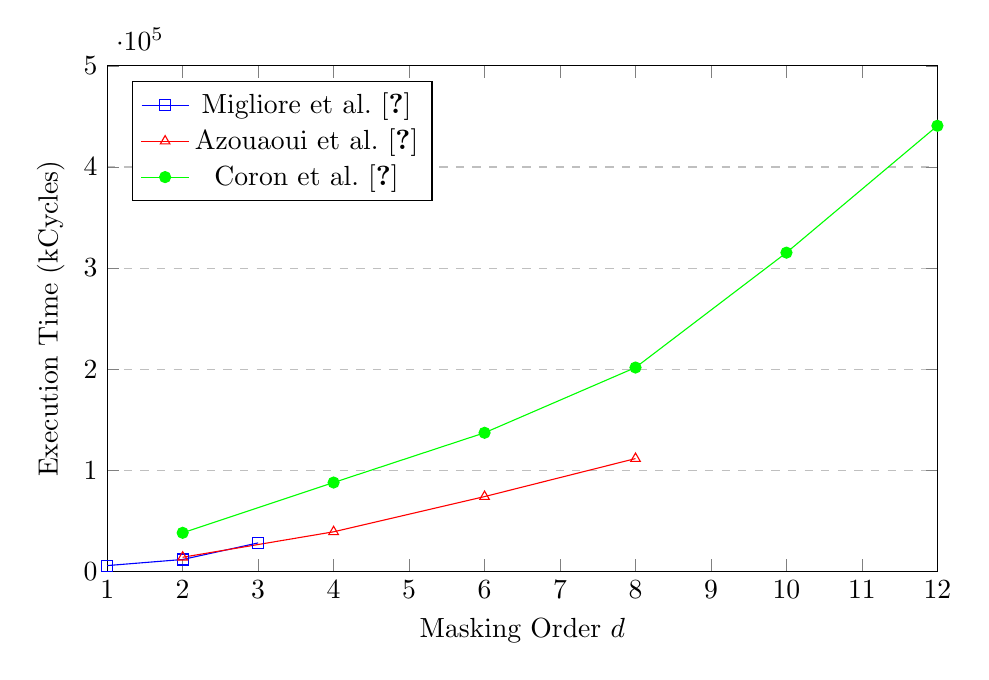
\begin{tikzpicture}
        \begin{axis}[
                xlabel={Masking Order $d$},
                ylabel={Execution Time (kCycles)},
                xmin=1, xmax=12,
                ymin=0, ymax=500000,
                xtick={1,2,3,4,5,6,7,8,9,10,11,12},
                ytick={0,100000,200000,300000,400000,500000},
                legend pos=north west,
                ymajorgrids=true,
                grid style=dashed,
                width=\textwidth,
                height=8cm,
            ]

            % Migliore et al.
            \addplot[
                color=blue,
                mark=square,
            ]
            coordinates {
                    (1, 5.64*1000)
                    (2, 11.68*1000)
                    (3, 28.08*1000)
                };
            \addlegendentry{Migliore et al.~\cite{Migliore19}}

            % Azouaoui et al.
            \addplot[
                color=red,
                mark=triangle,
            ]
            coordinates {
                    (2, 13891.4)
                    (4, 39064.5)
                    (6, 73905.4)
                    (8, 111515.4)
                };
            \addlegendentry{Azouaoui et al.~\cite{Azouaoui22}}

            % Coron et al.
            \addplot[
                color=green,
                mark=*,
            ]
            coordinates {
                    (2, 38069)
                    (4, 87809)
                    (6, 137034)
                    (8, 201583)
                    (10, 315249)
                    (12, 440769)
                };
            \addlegendentry{Coron et al.~\cite{Coron23}}

        \end{axis}
    \end{tikzpicture}
    \caption{Execution Time of Masked Signing Operation at Different Masking Orders}
    \label{fig:scalability}
\end{figure}
\newpage

Migliore et al.'s approach is practical for lower masking orders but may become less feasible at higher orders, especially due to the non-standard modulus. In contrast, Azouaoui et al.'s implementation demonstrates better scalability, with execution times increasing moderately due to their optimized gadgets and use of randomized signing. Coron et al.'s implementation supports masking orders up to $d=12$, but with significant performance overhead at higher orders.

\section{Feasibility on Embedded Devices}

Feasibility on embedded devices depends on achieving acceptable performance within the limited computational resources available. Table~\ref{tab:feasibility} summarizes the feasibility considerations for each implementation.

\begin{table}[h]
    \centering
    \renewcommand{\arraystretch}{1.2}
    \caption{Feasibility of Implementations on Embedded Devices}
    \begin{tabular}{l | p{10cm}}
        \toprule
        \textbf{Implementation}           & \textbf{Feasibility Considerations}                                                                                                                                                                                                                                                      \\
        \midrule
        Migliore et al.~\cite{Migliore19} & Feasible for first-order masking on embedded devices due to moderate overhead. The use of a power-of-two modulus simplifies computations and improves performance. Higher masking orders (beyond $d=3$) may be less practical due to increased overhead and modifications to the scheme. \\
        \midrule
        Azouaoui et al.~\cite{Azouaoui22} & Feasible for higher-order masking up to $d=8$ on devices like ARM Cortex-M4. Optimizations and the use of randomized signing reduce the overhead, making it practical for embedded devices even at higher security levels.                                                               \\
        \midrule
        Coron et al.~\cite{Coron23}       & Feasible at lower masking orders, but high execution times at higher orders may exceed the capabilities of typical embedded devices, limiting practicality. The implementation's complexity increases with $d$, affecting scalability on resource-constrained platforms.                 \\
        \bottomrule
    \end{tabular}
    \label{tab:feasibility}
\end{table}

Azouaoui et al.'s implementation is particularly suitable for embedded devices even at higher masking orders due to their efficient masking techniques and optimizations. Migliore et al.'s approach is practical for lower masking orders but may become less feasible at higher orders and due to the non-standard modulus. Coron et al.'s implementation may be challenging to deploy on embedded devices at higher masking orders due to increased complexity and resource demands.

\section{Implementation Techniques and Optimizations}

The specific techniques and optimizations employed significantly impact the security and performance of the implementations. Table~\ref{tab:implementation_techniques} highlights the key techniques used by each implementation.

\begin{table}[h]
    \centering
    \renewcommand{\arraystretch}{1.2}
    \caption{Implementation Techniques and Optimizations}
    \begin{tabular}{l | p{11cm}}
        \toprule
        \textbf{Implementation}           & \textbf{Techniques and Optimizations}                                                                                                                                                                                                                                                                                                                                              \\
        \midrule
        Migliore et al.~\cite{Migliore19} & Use of power-of-two modulus to simplify masking, specialized algorithms for masking polynomial arithmetic, focus on minimizing non-linear operations. The power-of-two modulus allows for efficient masking of decomposition functions and reduces complexity of arithmetic-to-Boolean conversions.                                                                                \\
        \midrule
        Azouaoui et al.~\cite{Azouaoui22} & Refined sensitivity analysis correcting previous flaws, development of new masking gadgets tailored for Dilithium, use of Probe-Isolating Non-Interference (PINI) compliant gadgets, exploitation of randomized signing to reduce overhead by avoiding costly masked deterministic functions like Keccak. Optimizations in sampling and arithmetic operations enhance performance. \\
        \midrule
        Coron et al.~\cite{Coron23}       & Introduction of new efficient masking gadgets (e.g., ShiftMod gadget), optimized algorithms for high-order masking, security proofs in the probing model, focus on arithmetic modulo operations. Their gadgets reduce the complexity of critical operations at small masking orders but have exponential complexity growth with $d$.                                               \\
        \bottomrule
    \end{tabular}
    \label{tab:implementation_techniques}
\end{table}

Azouaoui et al.\ introduce several optimizations, including refined sensitivity analysis and new masking gadgets, which enhance both security and performance. The use of randomized signing avoids the need to mask complex deterministic functions, further reducing overhead. Migliore et al.\ optimize their implementation by simplifying the modulus to a power-of-two, which significantly eases the masking of decomposition operations and reduces the number of non-linear operations. Coron et al.\ focus on creating efficient gadgets for high-order masking and provide strong security proofs, but the complexity increases with the masking order.
\newpage

\section{Trade-offs Between Security and Performance}

Implementing higher-order masking increases security but also introduces significant performance overhead. Each implementation addresses this trade-off differently:

\begin{itemize}
    \item \textbf{Migliore et al.~\cite{Migliore19}} prioritize performance at lower masking orders by simplifying the modulus to a power-of-two, which may affect compliance with standard parameters and security proofs. While efficient at first-order masking, higher orders result in substantial overhead, and the non-standard modulus may pose challenges for interoperability and security assurance.
    \item \textbf{Azouaoui et al.~\cite{Azouaoui22}} aim for a balance between high security and reasonable performance by introducing optimized gadgets and using randomized signing, making higher-order masking practical. Their approach maintains compliance with standard parameters and avoids modifications to the scheme.
    \item \textbf{Coron et al.~\cite{Coron23}} focus on providing strong security proofs for high-order masking, accepting higher performance overheads as a trade-off for increased security. The exponential complexity with higher $d$ values limits scalability on embedded devices but may be acceptable in contexts where strong security guarantees are required.
\end{itemize}

\section{Synthesis, Discussion, and Conclusion}

Our comparative analysis shows that Azouaoui et al.'s implementation offers the most practical balance between security and performance for embedded devices, supporting higher-order masking up to $d=8$ with reasonable execution times. Their optimizations and use of randomized signing make higher-order masking feasible in resource-constrained environments.

Migliore et al.'s implementation is suitable for applications where lower-order masking suffices and modifications to the modulus are acceptable. They achieve good performance improvements through modulus simplification, but the use of a power-of-two modulus deviates from standard parameters, which may raise compatibility and security concerns.

Coron et al.'s implementation provides strong security assurances through high-order masking and formal proofs, but the associated performance overhead may limit its practicality on embedded devices. It is more suited for scenarios where security is paramount and resources are less constrained.

In conclusion, the choice of implementation depends on the specific security requirements and resource constraints of the target application. For embedded devices requiring high levels of side-channel resistance without altering the standard scheme, Azouaoui et al.'s approach is recommended due to its optimized balance of security and performance. Migliore et al.'s implementation can be considered when performance is critical and lower-order masking is sufficient, keeping in mind the potential issues with non-standard parameters.

% References (ensure the references are correctly cited in your bibliography)
% \bibliographystyle{plain}
% \bibliography{bibliography}

% End of comparative_analysis.tex